\chapter{The Library}

\vspace{1em}
\hfill
\begin{minipage}[c]{0.55\textwidth}
\raggedleft
\small\itshape
The universe (which others call the Library) is composed of an indefinite, perhaps infinite number of hexagonal galleries.\\[0.5em]
\upshape\footnotesize Jorge Luis Borges, \textit{The Library of Babel} (1941)
\end{minipage}%
\hspace{0.5em}
\begin{minipage}[c]{0.12\textwidth}
% \includegraphics[width=\textwidth]{figures/ch02_library.png}
\end{minipage}
\vspace{1.5em}

\noindent In 1941, Jorge Luis Borges described a library.

The library contains every possible book. Every book is the same physical size: 410 pages, 40 lines per page, 80 characters per line, drawn from an alphabet of 25 symbols. The total number of distinct books is finite but enormous, roughly $25^{1{,}312{,}000}$.\footnote{This is a real number. It is finite. It is also vastly larger than the number of atoms in the observable universe, which is about $10^{80}$. Borges' narrator was uncertain whether the library was infinite. The mathematics is not uncertain. The library is large, but it is not infinite.}

Most of the books are gibberish. Long runs of meaningless characters. Page after page of the letter $m$. A book that is the letter $e$ repeated one and a third million times. The library contains all of these, because they are possible.

But the library also contains every meaningful book. Every novel ever written. Every novel that could ever be written. Every history textbook, true and false. Every scientific paper, including the ones that have not yet been written. Every love letter you might send, and every love letter you might not. The book describing what you will do tomorrow, in correct detail. The book describing what you will do tomorrow, in incorrect detail. The catalog listing the locations of all true books. The catalog listing false locations of all true books.

The library contains everything that can be written.

\section*{Generating the library}

Pause on how cheap this is to specify.

You do not need to describe the library book by book. You need to describe a procedure: \emph{produce every possible string of 1,312,000 characters from a 25-symbol alphabet, and bind each one as a book}. Three lines of pseudocode. The entire library, in all its unfathomable size, is the output of a tiny program.

The procedure does not know what is in the books. It does not care whether a string is gibberish or genius. It produces all of them, indiscriminately. The library's totality is informationally trivial. The library's contents are inexhaustible.

This is the first hint. The thing that feels like the hard problem (the universe of all possible books) is not the hard problem. The thing that feels like the small problem (this book, the one you wanted) is the hard one.

\section*{Indexing}

Generation is trivial.

Indexing is everything.

In Borges' library, finding any specific book is the entire challenge. Not because the library is hidden. The library is, by hypothesis, fully laid out. Every book is on a shelf, at a specific gallery, at a specific position. The library is complete and accessible. What is missing is a way to point to the book you want.

A catalog would help. But the catalog is also a book, somewhere in the library. So is the catalog of catalogs. So is the catalog that lies about the locations of the true catalogs. You cannot find the catalog without already knowing where it is. The library contains the answer to every question, and the address of every answer, and the lie about the address of every answer. It contains the catalog that lists only true books, the catalog that looks like that catalog but is wrong in one position, the catalog that is wrong in two, and so on through every degree of corruption. Without a starting handle, you can search for centuries without retrieving anything but noise.

What you have, when you stand in front of a wall of identical-looking volumes, is a problem of \emph{indexing}: a way of picking out, from the totality of what could be written, the part that is relevant to where you are. The library is the space of possibility. You are an indexed point in it.

The naive picture would have it that the universe of possibilities is the mystery and your local situation is the small concrete fact. The library says the opposite. The universe of possibilities is the cheap thing. The local fact is the expensive thing. Information is in the cut.

\section*{From books to programs}

The same trick generalizes far beyond books.

Borges fixed his books at 410 pages. Let go of that constraint. Consider every possible computer program, of any length, in any reasonable programming language. The space of all such programs is, again, trivial to specify. Programs are finite strings of symbols. You can enumerate them in order of length: one-symbol programs, then two-symbol programs, then three-symbol programs, and so on. The procedure is a few lines. The list goes on forever.\footnote{This kind of enumeration is the central object of computability theory. In 1936, Alan Turing showed that everything that can be computed at all can be produced by a single finite machine running through all programs in interleaved time-steps. The machine itself is a small object. What it can compute is the entirety of what is computable.} Figure~\ref{fig:enumeration-tree} shows the structure: every binary string of length $n$ is a leaf at depth $n$ in a binary tree.

\begin{figure}[h]
\centering
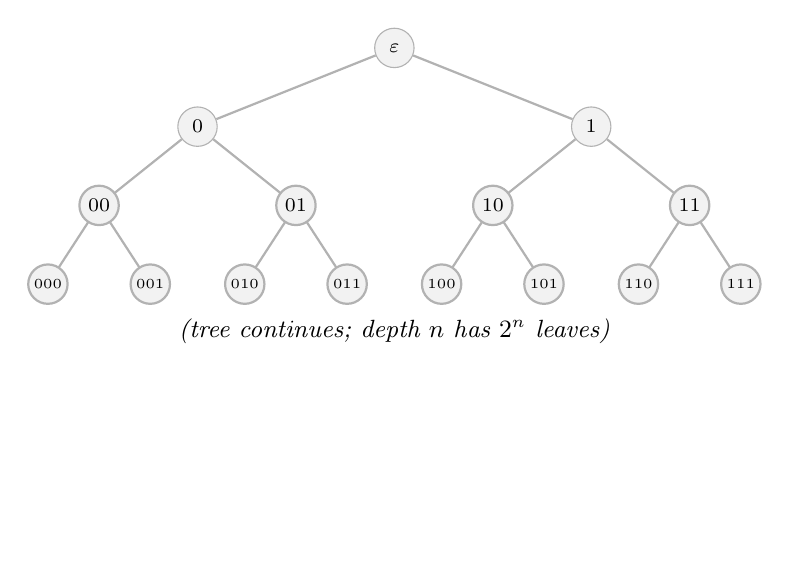
\begin{tikzpicture}[
  level distance=1cm,
  level 1/.style={sibling distance=5cm},
  level 2/.style={sibling distance=2.5cm},
  level 3/.style={sibling distance=1.3cm},
  edge from parent/.style={draw, thick, gray!60},
  every node/.style={circle, draw=gray!60, fill=gray!10, inner sep=1pt, minimum size=5mm, font=\scriptsize}
]
  \node {$\varepsilon$}
    child {node {0}
      child {node {00}
        child {node[font=\tiny] {000}}
        child {node[font=\tiny] {001}}
      }
      child {node {01}
        child {node[font=\tiny] {010}}
        child {node[font=\tiny] {011}}
      }
    }
    child {node {1}
      child {node {10}
        child {node[font=\tiny] {100}}
        child {node[font=\tiny] {101}}
      }
      child {node {11}
        child {node[font=\tiny] {110}}
        child {node[font=\tiny] {111}}
      }
    };

  \node[draw=none, fill=none, font=\small\itshape] at (0, -3.6) {(tree continues; depth $n$ has $2^n$ leaves)};
\end{tikzpicture}
\caption{The library of all binary strings, generated by descending a binary tree. One rule produces the entire structure: branch on $0$ or $1$ at each step. Strings of length $n$ live at depth $n$. Generation is trivial: descend the tree. Locating any specific string requires its full path, $n$ bits of address for a string of length $n$. The cost of the generator is constant. The cost of an address grows with depth.}
\label{fig:enumeration-tree}
\end{figure}

Most programs are not valid syntax. Most of the valid ones do not halt. Some of them, when run, produce coherent output: numbers, sequences, images, behaviors. A vanishingly tiny fraction produce output that looks like an actual physical process. A still tinier fraction look like the universe you observe.

All of these programs already exist in the enumeration. The enumeration is one rule. Running them produces every possible computable sequence. Every weather pattern, every chess game, every fictional history, every real one. The program that draws a galaxy. The program that simulates a galaxy. The program that simulates a universe with slightly different physical constants. The program that produces your visual cortex's response to morning light. The program that produces a universe identical to yours, except for one molecule. The program that has read a trillion words of human writing and predicts the next one. The program that produces this book.

The library of books is small. The library of programs is the larger structure of which the library of books is one tiny shelf.

The space of all programs is cheap. Locating the specific program whose output matches your data is the hard problem. ``Where am I in the library of programs'' has the same shape as ``where am I in Borges' library.'' The library is larger; the question is the same.

\section*{A note on the metaphor}

The library of books, the library of programs, the enumeration tree: each decomposes the totality into discrete items, neatly numbered. The decomposition is convenient. The rest of this book often speaks this way. But the underlying structure does not require it. Any regularity in the bit-sequences is exploitable by some program; programs can share substructure across what we call separate items. The decomposition into ``books'' or ``programs'' is the cartographer's tool, not a feature of the territory.

When this book uses \emph{index} or \emph{book} or \emph{coordinate}, the discreteness is a working approximation. The label is on the structure, not in it. Chapter 13 returns to this seriously, in parallel with the dissolution of the self.

\section*{Empty and universal}

There is a way to make the cheapness of the totality sharper still.

Consider the empty set: the collection that contains nothing. You can describe it in one symbol: $\emptyset$. Now consider the universal set: the collection that contains everything. You can describe it in one phrase: \emph{everything}.

Both are easy to write down. Both are short to specify. The empty set is cheap because there is nothing to enumerate. The universal set is cheap because the enumeration is too long to perform, and you sidestep it by referring to the totality. Either extreme is, informationally, almost free.

The expensive descriptions are the ones in the middle. The set of all books that are coherent. The set of all programs whose output matches your observations. The set of all configurations of matter that constitute the inside of your living room. Each of these is a subset of the universal set, and each one requires substantial information to specify, because each one is a particular cut.

A theory that explains \emph{everything} explains nothing. A theory that explains \emph{nothing} explains nothing. A theory that explains \emph{this} is the only interesting thing. The act of explanation is the act of indexing.

\section*{Where this leaves you}

Step back.

You are an observer with data. Your data is, like the chicken's, a small finite slice of a vastly larger structure. The structure is, like Borges' library, cheap to specify in its totality and expensive to navigate. Given your data, what is the right way to point to where you are in the structure?

This is the indexing question. You have been answering it your whole life, under another name.

It is called probability.
